\svnidlong
{$HeadURL: svn+ssh://blanqui@scm.gforge.inria.fr/svnroot/simsoc-cert/papers/itp13/simsoc-cert.tex $}
{$LastChangedDate: 2013-04-18 13:09:21 +0200 (jeu. 18 avril 2013) $}
{$LastChangedRevision: 2302 $}
{$LastChangedBy: monin $}

% Author: \svnfileauthor; Revision: \svnfilerev; Last changed on: \svnfiledate; 
% URL: \url{\svnkw{HeadURL}}

\begin{thoughts}
\itshape
\hfil -----------------------------------------------------------------------------------\par
\hfil \textbf{Changes on \currfilename}

Author: \svnfileauthor; Revision: \svnfilerev; Last changed on: \svnfiledate
\end{thoughts}

% svn propset svn:keywords 'LastChangedBy LastChangedRevision LastChangedDate HeadURL' thisfile.tex

%%%%%%%%%%%%%%%%%%%%%%%%%%%%%%%%%%%%%%%%%%%%%%%%%%%%%%%%%%%%%%%%%%%%%%%%%%%%%
\section{Application to SimSoC-cert}
\label{sec:simsoccert}

SimSoC-Cert~\cite{rapido11,cpp11} aims at certifying the simulator SimSoC, 
which is a complex hardware simulator written in C and C++.
SimSoC is able to simulate various architectures including ARM and SH4 and is 
efficient enough to run Linux on them at a realistic speed.
The main objective of SimSoC is to help designers of embedded systems:
a large part of the design can be performed on software,
which is much more convenient, flexible and less expensive
than with real specific hardware components.
However, 
this only makes sense if the simulator is actually faithful to the real
hardware.
Therefore we engaged in an effort to provide a formal certification
of sensitive parts of SimSoC.
More precisely, we consider the Instruction Set Simulator (ISS)
for the ARM, which is at the heart of SimSoC.
This ISS is called Simlight.

To this effect, first we defined a formal model in Coq of the ARM architecture,
as defined in the reference manual~\cite{arm6refman}.
% This is essential for defining the reference expected behavior of SimSoC. % could be kept if enough room
Our second input is the operational semantics of the ISS encoded in C. 
This program is actually written in a large enough subset of C
called Compcert-C,
which is fully formalized in Coq \cite{Leroy-Compcert-CACM}.

We can then compare the behavior of the ISS encoded in C 
with the expected reference model directly defined in Coq.
To this effect, a projection between the Coq model of the
memory state of Simlight to the states in the reference model
is defined.
Then, correctness statements express that from a 
C memory $m_1$ corresponding to an abstract state $s_1$,
performing the function claimed to represent a given instruction $\cal I$
in Simlight 
will result in a C memory $m_2$ which actually corresponds 
to the abstract state $s_2$ obtained by
running the Coq model of $\cal I$. 
This can be put under the form of a commutative diagram as
schematized in Fig.~\ref{fig:thrm}.
%% HERE THE FIGURE 

\begin{figure}
\hfil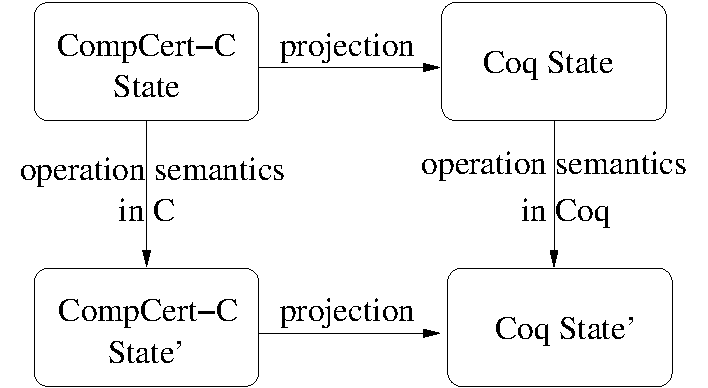
\includegraphics[width=.5\linewidth]{theorem.pdf}
\caption{Correctness of the simulation of an ARM operation}
\label{fig:thrm}
\end{figure}

% Using the CompCert defined operational semantics for program
% correctness proof requires quite a lot of interactive efforts. 
% For a system complicated like this, a full system simulation with a complete
% instruction set simulation, the specification is very detailed
% describing a processor state transistion system.  
% The theorem is stated relying on CompCert operational semantics.
The operational semantics of C defining the evaluation is used everywhere 
in the proof: it provides the decomposition of the vertical arrow
on the left column of Fig.~\ref{fig:thrm} 
and drives the proof accordingly. %  sequences steping forward.  
%
We use the big step semantics, 
which is defined in CompCert by 5 mutually inductive transition relations.
The largest inductive type for the evaluation of C expressions 
is \coqdocvar{eval\_expr}.
It has 17 constructors, one for each CompCert C expression 
such as assignment, binary operation, dereference, etc.  
% Since each ARM instruction operation is defined by a sequence of quite
% complex statements which can be decomposed into many single expressions.

% A typical proof step starts with an intuitive goal, 
% stating that a pair of C memory states are related 
% by one or several expressions. 
% To reveal the relation between the two memory states is the first target. 

In a typical proof step, 
we start from a goal containing 
a conclusion stating that 
a C memory state $m_n$ and an ARM state $st_n$ in the reference model 
are related by our projection,
a hypothesis $R_0$ stating a similar relation between 
a C memory state $m_0$ and an ARM state $st_0$,
and additional hypotheses $He_1, He_2, \ldots, He_n$.
relating pairs of successive C memory states 
$(m_0, m_1)$, $(m_1, m_2), \ldots, (m_{n-1}, m_n)$
respectively with (ASTs for) C expressions $e_1$, $e_2, \ldots,$ $e_n$,
according to the relevant transition relation provided by CompCert.
The general strategy is to propagate information
from $m_0$ to $m_1$ using $R_0$ and $He_1$, 
then so on until $m_n$.
To this effect we invert $He_1$, $He_2$, etc.
However, according to the structure of $e_1$, 
inverting $He_1$ generates intermediate memory states
and corresponding hypotheses that have to be inverted before 
going to $He_2$, unless $e_1$ is a base case.
And sometimes, other kind of reasoning steps are needed,
e.g., lemmas on the reference model of ARM.

% Then such hypothesis need to be inverted according
% to its inductively defined definition. 
% The result of inverting should either yields more permises 
% for these two memory state or finally
% tells the memory states are equivalent. 
% The new given permises could be again elementary transitions 
% between those states.  

% And the drawblack is very obvious here by using the Coq build-in tactic \inversion. 

%In detail,
%changes in the C memory model are formally described
%by a transition system according to the operational semantics of Compcert-C.
%Therefore, the later is  used everywhere in the proofs. 
%This operational semantics is described by
%a big mutual inductive type;
%in particular, the evaluation of expressions is defined by
%16 constructors, one for each CompCert C expression such as assignment or binary
%operation.
%% And this inductive type evaluation of expression is our target to try the
%% improved new inversion.
%A typical proof step starts from a goal intuitively saying that,
%given two C memory states related by a C expression,
%as expressed in some hypothesis $H$, 
%some commutative diagram holds.
%Then $H$ is inverted, which either yields more elementary 
%transitions between C memory states, 
%with corresponding expected commutative diagrams,

%or solves the current diagram if the considered expression
%is atomic. 
%In general we see that an inversion will result in many
%new opportunities to perform inversions.

%In our first proofs, using the Coq standard \inversion tactic
%resulted in a very weak control on the script.
%Finding the right relation to focus on in the hypotheses
%was inconvenient.
%Interactive execution of the script was also quite slow,
%due to the size of the terms generated by \inversion.
%And the compilation time for the proof on only one instruction 
%took more than one minute --
%there are more than one hundred instructions in the ARMv6 architecture.
%Moreover
%the proof code is fragile in case of changes: 
%after \inversion, hypotheses are automatically given similar names 
%according to a simple numbering scheme,
%so that any modification at the beginning of the proof script
%or in auxiliary lemmas 
%result in a complete renaming of hypotheses to come in the sequel.
%This is quite harmful in practice and constitutes
%a serious issue for maintenance.

For illustration,
the following code shows a small excerpt from an old proof script in
SimSoC-Cert using \inversion. 
It corresponds to one line taken in an instruction called ADC (add with carry).
It sets the CPSR (Current Program Status Register) with the value of SPSR 
(Saved Program Status Register). 
Lemma $same\_cp\_SR$ states that 
the C memory state of the simulator and 
the corresponding formal representation of ARM processor state 
evolve consistently during this assignment.
The pseudo-code from the ARM reference manual is just $CPSR~=~SPSR$.
The corresponding C code is represented by the identifier $cp\_SR$ 
in the statement of the lemma.

\coqdocinput{chunk43}

\medskip\noindent
After a couple of introductions and other administrative steps,
we get the following goal,  
where $cp\_SR$ is unfolded in hypothesis $H$.

%\coqdocinput{chunk45}

\medskip
\dots \\
\hspace*{-1.7mm}
\coqdocinput{chunk41}

\noindent
Then we have to invert $H$ and similar generated hypotheses
until all constructors used in it type are exhausted. 
Here 18 consecutive inversions are needed.
Using \inv, which performs standard \inversion, clearing 
the inverted hypothesis and rewriting of all auxiliary equations,
the sequel of the script started as follows.
% To make use of hypothesis $H$, We see inside the proof many \inv are
% used.  Here \inv denoted three proving tactics \coqdocvar{inversion H;
%   clear H; subst}: inverting the hypothesis, delete the useless
% original hypothesis, and substitutions.  We chose to use \inv tactics
% to save developement time without providing names and such combined
% tactic is easy to write.  Then the problem arrived, it is not possible
% to understand the proof just reading a list of \inv, even for the
% writer who wrote them a while ago.

\medskip
\coqdocinput{chunk42}
\medskip

\noindent
The names used there ($H4$, $H9$, etc.) are not under our control.
The program for simulating an ARM
instruction usually contains expression more complex than in the
example given here.
% This cumbersome work is needed in correctness proofs for every instruction,
And unfortunately there is no clear way to share parts of the proofs
involved since the corresponding programs are rather specific,
at least for instructions belonging to different categories.

The drawbacks of the standard tactic \inversion presented
in the introduction show up immediatly.
%
A first clue is the response time of Coq when inverting hypotheses $H_i$.
Compiling the proof script corresponding to one instruction
took more than a minute.
%
% Second, maintaining the proof scripts is harder than expected. 
% The proof code is fragile, 
% once a modification is required inside proving, from that point
% to the end the proof stradegy need to be modified all over again.
% Because applying the build-in \inversion itself will automatically
% name the new introduced elements. And the following script will refer
% to some of these names. 
%
% The naming algorithm of build-in \inversion just uses index for hypothesis, 
% then reading the code without any comments is not possible to understand the meaning of each step. 
% And a small modification may change the order of naming all the following
% hypotheses.  If we use \inversion with option, in order to have name
% controls, the other problem will be raised due to the size of the
% targeting inductive type of the hypotheses. 
%
% As we mentioned before,
% the inductive type which representing the evaluation has a lot of
% constructors which are all well-detailed.  
%
About the naming issue, 
the constructors we face have up to 19 variables and 6 premises,
yielding 25 names to provide.
We could try to automate this naming using an ad-hoc wrapper 
around \inversion, 
but things are complicated by 
the fact that this inversion program inserts
additional hypotheses putting equational constraints 
between variables of the inverted constructor.
There are different ways to state and to place such constraints,
and different releases of Coq may make different choices.
The BasicElim approach introduces equations as well
but from on our experiments, 
generated goals are much more regular than with \inversion.
In contrast, 
our approach does not suffer from such interferences,
so we are anyway in a better position. 

% Therefore, 
% inverting a hypothesis corresponding to this case yields 25 names to give.
% And due to the complexity of an expression. 
% Such \inversion with option of naming
% control need to apply for many times. Then giving names to 25 elements
% will be repeated for times. It is absolutly a very boring work.

% Then the hand crafted tactic should be able to deal with the two problem
% above, and also be robust enough against the changing of proof
% environment.  The following will detailed all the effort we have
% performed for SimSoC-Cert project rely on our ad-hoc inversion tactic
% presented in the last sections.

% Thanks to the technique introduced in this paper, we could define
% convenient reusable tactics. 
First, we define the diagonal-based function for each constructor 
of $eval\_expr$, following the lines given in the previous section.
For example, 
the evaluation of a field is defined in CompCert by the following rule.

\medskip
\coqdocinput{chunk50}
\medskip

\noindent
We then define (observe that 2 variables and 1 hypothesis will be generated):

\medskip
\coqdocinput{chunk52}
\medskip

% An interesting one, for expression $val\_of$, 
% has it inversion function defined as follows.
%
% \medskip
% \coqdocinput{chunk40}
% \medskip
%
% % It is fully depended on the constructor $eval\_valof$ definition. The
% % implicit arguments of $inv\_valof$ are the references helps us to
% % indicate the the object hypothesis. 
% $inv\_valof$ is special, because the memory access can be volatile or not,
% so that inverting the hypothesis of type $eval\_valof$ returns two cases,
% whereas we get only one case for all other constructors.
% Using the impredicative encoding here in the diagonal function
% can achieve the same casing effect. If type of the expression is
% volatile, we have to evaluate such expression again to get the
% reduction result, then ask for the volatile type to perform the same
% process all over.

%Thanks to the technique introduced in this paper,
%we could define convenient reusable tactics.
%First, we defined suitable diagonal-based functions for each
%constructor of $eval\_expr$ following the lines given in the
%previous section.

% As we showed in the example above, the old way of inverting hypotheses is a 
% repetitive work. To get the relation of memory states between a not too
% complex expression requires 18 \inv. 
% After we changed to the new inversion,
% we still need 18 corresponding ad-hoc inversions for every decomposed
% expression.
Next we introduce a high-level tactic 
% aiming such problem happened in SimSoC-Cert project. 
for each inductive type, gathering all the functions defined for 
its constructors. % and solve the heavy and repetitive naming trouble. 
For example, $eval\_expr$ contains:

\medskip
\coqdocinput{chunk51}

\noindent
This tactic has two arguments $m$ and $m'$, corresponding to C memory states.
The first \texttt{intros} introduces the 3 generated components 
with names respectively prefixed by \coqdoccst{t}, \coqdoccst{v} and \coqdoccst{ev\_ex}.
The second \texttt{intros} is related to previously reverted 
hypotheses, their names are correctly managed by Coq.
Alltogether, such a tactic will:
\begin{enumerate}
\item Automatically find the hypothesis matching the arguments to be inverted;
\item Repeatedly perform our hand-crafted inversions for type
  $eval\_expr$ until all constraints between two memory states $m$ and
  $m'$ are derived;
\item Give meaningful names to the derived constraints;
\item Update all other related hypotheses according to the new 
  variable names or values;
\item Clean up useless variables and hypotheses.
\end{enumerate}
%

%Then we packaged them together in a high-level tactic named 
%$inv\_eval\_expr$ using an Ltac definition. The arguments of this
%tactic are the memory states under focus --
%in the example above: $m$ and $m'$.
%This tactic also contains extra features so that
%it is able to:
%%
%\begin{enumerate}
%\item automatically find an hypothesis to be inverted;
%\item repeatedly perform our hand-crafted inversion until all constraints
%  between two memory states are derived;
%\item give meaningful names to the derived constraints;
%\item update all other related hypotheses according to the new 
%  variable names or values;
%\item clean up useless variables and hypotheses.
%\end{enumerate}
%%
\noindent
For example the 18 \inv in the example above are solved in 
one step using $inv\_eval\_expr~m~m'$, 
Note that the names are not explicitly given in the script,
which would be cumbersome,
but generated in our tactic.

% Defining such high-level tactics is aim to avoid repetitively naming issue
% we mentioned, the real killer in our developement of correctness proof.
% Like constructor $eval\_valof\_volatile$ in type $eval\_expr$ requires 17
% names to give if we want this full control. 
% Using the ad-hoc tactics like $inv\_eval\_expr$ requires no name to
% give to variables or hypotheses.The names are given during defining
% %the general hc\_inversion, according to the meaning of the hypo
% %orwhatever names you can recognise later.For example, hypo
% the general \verb!hc_inversion!, \todo{a}{newcommand for hcinv}
% according to the meaning of the hypothesis
% or whatever names you can recognise later. 
% For example, hypothesis
% $find\_funct~ge~vf$ is named $Hfindfunc$. When maintaining the scripts,
% we know which hypo it refers to. It is done once for all. Unlike using
% build-in inversion, you don't need to look at the big inductive
% definition for the long list of variables and premises every time you
% apply inversion. The naming stradegy used in this kind of high-level tactic
% is semi automatic. We can have a better control by giving names according to
% the type of the hypotheses. But the names of hypotheses of the same type will
% be named with index at the end $Hfindfunc1$ $Hfindfunc2$. We have to compromise
% between making the tactic easy to apply with and even a better control on index.
% Here we prefer the tactic to be simple and easy to use.

% \todo{r}{BEGIN to be removed -- or moved to intro}%
% To be fair, let us mention that the robustness issue could,
% in principle, be managed using the current version of standard \inversion,
% because it allows us 
% to give explicit names to introduced variables and hypotheses.
% However, due to the complexity of CompCert C semantics, 
% providing all these names explicitly turns out to be cumbersome,
% and unrealistic when you face dozens of consecutive \inversion 
% and about ten names for each \inversion.
% \todo{r'}{END to be removed -- or moved to intro}%
% Within our framework,
% the introduction of suitable names
% is automatically performed inside $inv\_eval\_expr~m~m'$.
% Names are chosen according to the contents and in a flexible way, 
% so that the evolution of goals is easy to follow.

Coq version changes had no impact on our scripts.
Unexpectedly, 
changes in CompCert C semantics between versions 1.9 and 1.11
had no impact as well on proof scripts using our inversion.
Of course, we still had to update the definition of diagonal functions. 
% In the proof script, the step for inverting on an inductive type will
% always uses its specific ad-hoc inversion without any change. 
% But the changes in the script may happen, if the following step refers to
% some new derived elements.

Comparing development times provides additional hints.  
In our first try, using built-in inversion,
more than two months were spent (by one person) on the development of 
the correctness proof of instruction ADC.
Much time was actually wasted at maintaining the proofs since,
as mentioned, a little change resulted in 
a complete revision of proof scripts. 
% That's one of the important argument we need this ad-hoc inversion to be apply in SimSoC-Cert project.  
We then designed the inversion technique presented here.
% was not available at that time, entailing the drawbacks detailed above.  
With the new approach, proofs for 4 other simple instructions 
could be finished in only one week, 
taking of course advantage of the previous experience with ADC.
The high-level tactic described above required less than 2 weeks.

Finally, let us compare the efficiency of Coq built-in inversions 
(\inversion, 
\derive \inversion which can generate an inversion principle once for all, 
and BasicElim~\cite{mcbride00}) with our inversion.
We apply the four methods to the same examples, the lemma $cp\_SR$ and
a single inversion on type $eval\_expr$ from CompCert C semantics.
% Finally, we compare the efficiency of the standard Coq \inversion with
% our new tactic in Table.~\ref{t:timing}.  
The first row is about the whole expression given in the example above. 
The other rows are inversions of specific expressions: 
$Ecall$ is the CompCert-C expression of function calls, 
$Evalof$ is to get the value of the specified location, 
$Eval$ is to express constant, and $Evar$ is to express variables.  
We can observe a gain of about 4 to 5 times.
And generated object files are 5 times smaller.
%And compilation generates object files which are 5 times smaller.

% Finished transaction in 1. secs (1.428089u,0.024001s)
% Finished transaction in 0. secs (0.31202u,0.s)
% Finished transaction in 2. secs (1.628102u,0.s)
% Finished transaction in 1. secs (0.976061u,0.020001s)


\begin{table}\centering
\label{t:timing}
\caption{Time costs (in seconds)}
\begin{tabular}{|l|c|c|c|c|}
\hline
 & standard \inversion & \derive \inversion & BasicElim & our inversion \\
\hline
%Full example & 1.628102 & 0.976061 & 1.428089 & 0.31202 \\
Full example & 1.628 & 0.976 & 1.428 & 0.312 \\
\hline
%Ecall & 0.132009 & 0.076004 & 0.112007 &  0.028002\\
Ecall & 0.132 & 0.076 & 0.112 &  0.028\\
\hline
%Evalof &  0.132008 & 0.072004 & 0.092005 & 0.020001\\
Evalof &  0.132 & 0.072 & 0.092 & 0.020\\
\hline
%Evar &  0.128008 & 0.064004 & 0.084006 & 0.024001\\
Evar &  0.128 & 0.064 & 0.084 & 0.024\\
\hline
%Eaddrof &  0.140009 & 0.076005 & 0.104007 & 0.020001\\
Eaddrof &  0.140 & 0.076 & 0.104 & 0.020\\
\hline
\end{tabular}
\end{table}

% -rw-rw-r-- 1 xiaomu-shi xiaomu-shi  36712 Feb  5 19:50 comparison_ahinv.vo
% -rw-rw-r-- 1 xiaomu-shi xiaomu-shi 170821 Feb  5 19:50 comparison_basicelim.vo
% -rw-rw-r-- 1 xiaomu-shi xiaomu-shi 191346 Feb  5 19:50 comparison_inv.vo
% -rw-rw-r-- 1 xiaomu-shi xiaomu-shi 459613 Feb  5 23:40 comparison_derinv.vo


\begin{table}\centering
\label{t:size}
\caption{Size of compilation results (in KBytes)}
\begin{tabular}{|l|c|c|c|c|}
\hline
 & standard \inversion & \derive \inversion & BasicElim & our inversion \\
\hline
%Full example & 191346 & 459613 & 170821 & 36712\\
Full example & 191 & 460 & 171 & 37\\
\hline
\end{tabular}
\end{table}

%%% Local Variables: 
%%% mode: latex
%%% TeX-master: "itp13"
%%% End: 
